% Use texorpdfstring to handle emojis in TOC but safely in PDF bookmarks
\chapter{\texorpdfstring{\scalebox{2}{\twemoji{evergreen tree}} Trees \scalebox{2}{\twemoji{evergreen tree}}}{Trees}}

\section{Introdction}
The intuition for graph theoretic trees comes from actual trees in nature. Here, the stem splits into several branches that afterwards never rejoin.

% 3.1 Definition

\begin{definition}
A graph which does not contain cycles is called \textbf{\color{red}acyclic}.
We call a graph $G$ a \textbf{\color{red}tree} if it is connected and acyclic. An arbitrary acyclic graph is called a \textbf{\color{red}forest}.
In a forest, any vertex of degree 1 is called a \textbf{\color{red}leaf}.
\end{definition}

% 3.2 Remark
\begin{remark}
\begin{enumerate}
    \item[1)] The graphs $P_n$, $K_1$, $K_2$ and $K_{1,n}$ are trees for any $n \in \mathbb{N}$.
    \item[2)] Every tree is a forest.
    \item[3)] Every connected component in a forest is a tree.
    \item[4)] Every subgraph of a forest is a forest.
\end{enumerate}
\end{remark}

% 3.3 Example
\begin{example}
\begin{enumerate}
    \item[1)] 
    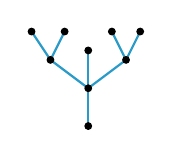
\begin{tikzpicture}[dot/.style={circle, fill=black, inner sep=0pt, minimum size=3pt},
        connector/.style={cyan!80!black, thick},
        baseline=-0.5ex, scale=0.6]
        % Tree: Root connected to a Hub. Hub splits into 3 branches.
        % Left/Right branches split again. Middle branch is a leaf.
        \coordinate (root) at (0,-0.8);
        \coordinate (hub) at (0,0);
        
        \coordinate (l) at (-0.8, 0.6);
        \coordinate (m) at (0, 0.8);
        \coordinate (r) at (0.8, 0.6);
        
        \coordinate (l1) at (-1.2, 1.2);
        \coordinate (l2) at (-0.5, 1.2);
        
        \coordinate (r1) at (0.5, 1.2);
        \coordinate (r2) at (1.1, 1.2);
        
        % Edges
        \draw[cyan!80!black, thick] (root)--(hub);
        \draw[cyan!80!black, thick] (hub)--(l);
        \draw[cyan!80!black, thick] (hub)--(m);
        \draw[cyan!80!black, thick] (hub)--(r);
        
        \draw[cyan!80!black, thick] (l)--(l1);
        \draw[cyan!80!black, thick] (l)--(l2);
        
        \draw[cyan!80!black, thick] (r)--(r1);
        \draw[cyan!80!black, thick] (r)--(r2);
        
        % Nodes
        \foreach \p in {root, hub, l, m, r, l1, l2, r1, r2} \filldraw (\p) circle (2pt);
    \end{tikzpicture}
    \textbf{\color{green!60!black}is a tree}.

    \item[2)]

    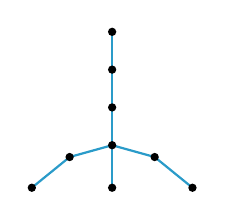
\begin{tikzpicture}[
        % Define styles for consistency
        dot/.style={circle, fill=black, inner sep=0pt, minimum size=3pt},
        connector/.style={cyan!80!black, thick},
        baseline=-0.5ex, scale=0.6
    ]

        % --- Coordinates ---
        % Central Hub
        \coordinate (hub) at (0,0);
        
        % Vertical Spine (going up)
        \coordinate (top1) at (0, 0.8);
        \coordinate (top2) at (0, 1.6);
        \coordinate (top3) at (0, 2.4);
        
        % Bottom Leg
        \coordinate (bot) at (0, -0.9);
        
        % Left Branch
        \coordinate (left_mid) at (-0.9, -0.25);
        \coordinate (left_end) at (-1.7, -0.9);
        
        % Right Branch
        \coordinate (right_mid) at (0.9, -0.25);
        \coordinate (right_end) at (1.7, -0.9);

        % --- Draw Edges (drawn first so they appear behind nodes) ---
        % Spine connections
        \draw[connector] (top3) -- (top2);
        \draw[connector] (top2) -- (top1);
        \draw[connector] (top1) -- (hub);
        
        % Bottom connection
        \draw[connector] (hub) -- (bot);
        
        % Left branch connections
        \draw[connector] (hub) -- (left_mid);
        \draw[connector] (left_mid) -- (left_end);
        
        % Right branch connections
        \draw[connector] (hub) -- (right_mid);
        \draw[connector] (right_mid) -- (right_end);

        % --- Draw Nodes ---
        \node[dot] at (hub) {};
        \node[dot] at (top1) {};
        \node[dot] at (top2) {};
        \node[dot] at (top3) {};
        \node[dot] at (bot) {};
        \node[dot] at (left_mid) {};
        \node[dot] at (left_end) {};
        \node[dot] at (right_mid) {};
        \node[dot] at (right_end) {};

    \end{tikzpicture}
    \textbf{\color{green!60!black}is a tree}.

    \item[3)]
    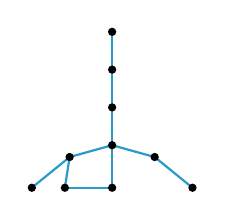
\begin{tikzpicture}[
        % Define styles for consistency
        dot/.style={circle, fill=black, inner sep=0pt, minimum size=3pt},
        connector/.style={cyan!80!black, thick},
        baseline=-0.5ex, scale=0.6
    ]

        % --- Coordinates ---
        % Central Hub
        \coordinate (hub) at (0,0);
        
        % Vertical Spine (going up)
        \coordinate (top1) at (0, 0.8);
        \coordinate (top2) at (0, 1.6);
        \coordinate (top3) at (0, 2.4);
        
        % Bottom Leg
        \coordinate (bot) at (0, -0.9);
        
        % Left Branch
        \coordinate (left_mid) at (-0.9, -0.25);
        \coordinate (left_end) at (-1.7, -0.9);
        
        % Right Branch
        \coordinate (right_mid) at (0.9, -0.25);
        \coordinate (right_end) at (1.7, -0.9);
        \coordinate (extra) at (-1, -0.9);

        % --- Draw Edges (drawn first so they appear behind nodes) ---
        % Spine connections
        \draw[connector] (top3) -- (top2);
        \draw[connector] (top2) -- (top1);
        \draw[connector] (top1) -- (hub);
        
        % Bottom connection
        \draw[connector] (hub) -- (bot);
        
        % Left branch connections
        \draw[connector] (hub) -- (left_mid);
        \draw[connector] (left_mid) -- (left_end);
        
        % Right branch connections
        \draw[connector] (hub) -- (right_mid);
        \draw[connector] (right_mid) -- (right_end);

        % Cycle connections
        \draw[connector] (left_mid) -- (extra);
        \draw[connector] (bot) -- (extra);

        % --- Draw Nodes ---
        \node[dot] at (hub) {};
        \node[dot] at (top1) {};
        \node[dot] at (top2) {};
        \node[dot] at (top3) {};
        \node[dot] at (bot) {};
        \node[dot] at (left_mid) {};
        \node[dot] at (left_end) {};
        \node[dot] at (right_mid) {};
        \node[dot] at (right_end) {};
        \node[dot] at (extra) {};

    \end{tikzpicture}
    \textbf{\color{red}is not a tree}.

    \item[4)]
    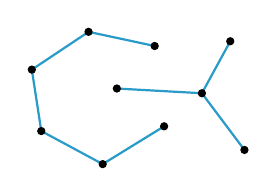
\begin{tikzpicture}[
        % Define styles
        dot/.style={circle, fill=black, inner sep=0pt, minimum size=3pt},
        connector/.style={cyan!80!black, thick},
        baseline=-0.5ex, scale=0.6
    ]

        % --- Coordinates ---
        
        % Left "C" Component
        \coordinate (left_back) at (-2.2, 0.5);
        
        % Top arch
        \coordinate (top_mid) at (-1.0, 1.3);
        \coordinate (top_tip) at (0.4, 1.0);
        
        % Bottom arch
        \coordinate (bot_mid) at (-2.0, -0.8);
        \coordinate (bot_low) at (-0.7, -1.5);
        \coordinate (bot_tip) at (0.6, -0.7);
        
        % Right "Y" Component
        \coordinate (center_tail) at (-0.4, 0.1);
        \coordinate (center_hub) at (1.4, 0.0);
        \coordinate (right_top) at (2.0, 1.1);
        \coordinate (right_bot) at (2.3, -1.2);

        % --- Draw Edges ---
        % Left component connections
        \draw[connector] (left_back) -- (top_mid);
        \draw[connector] (top_mid) -- (top_tip);
        \draw[connector] (left_back) -- (bot_mid);
        \draw[connector] (bot_mid) -- (bot_low);
        \draw[connector] (bot_low) -- (bot_tip);
        
        % Right component connections
        \draw[connector] (center_tail) -- (center_hub);
        \draw[connector] (center_hub) -- (right_top);
        \draw[connector] (center_hub) -- (right_bot);

        % --- Draw Nodes ---
        \node[dot] at (left_back) {};
        \node[dot] at (top_mid) {};
        \node[dot] at (top_tip) {};
        \node[dot] at (bot_mid) {};
        \node[dot] at (bot_low) {};
        \node[dot] at (bot_tip) {};
        \node[dot] at (center_tail) {};
        \node[dot] at (center_hub) {};
        \node[dot] at (right_top) {};
        \node[dot] at (right_bot) {};

    \end{tikzpicture}
    \textbf{\color{red}is not a tree}, but it \textbf{\color{green!60!black}is a forest}.
\end{enumerate}
\end{example}

% 3.4 Lemma
\begin{lemma}
Any tree of order at least 2 has at least two leaves.
\end{lemma}

\begin{proof}
Let $T$ be a tree with $|T| \ge 2$. In particular, $T$ is connected.
Consider a path of maximal length $P=(v_0, v_1, \dots, v_n)$ in $T$. As $|T| \ge 2$, we know that $v_0 \ne v_n$. We claim that $v_0$ and $v_n$ are leaves, i.e. $\deg(v_0)=\deg(v_n)=1$. We execute the argument for $v_0$.
As usual, we know that $N(v_0) \subseteq \{v_1, v_2, \dots, v_n\}$. Let $u \in N(v_0)$ arbitrary, i.e. $u=v_i$ for some $i \ge 1$. But then $(v_0, v_1, \dots, v_i, v_0)$ is a closed walk which is a cycle for all $i \ge 2$. As $T$ does not contain cycles, we conclude that $i=1$ and $v_1$ is the only neighbour of $v_0$. Hence $\deg(v_0)=1$ and $v_0$ is a leaf.
The argument for $v_n$ is analogous.
\end{proof}

% 3.5 Definition
\begin{definition}[Tree Pruning]
Let $T$ be a tree of order at least 3. We denote by \textbf{\color{red}$T^-$} the induced subgraph of $T$ obtained by deleting all leaves of $T$.
\end{definition}

% 3.6 Example
\begin{example}
\begin{enumerate}
    \item[1)] If $T=P_7$ the path of length 6, then $T^- = P_7^- = P_5$ is the path of length 4:
    \begin{center}
    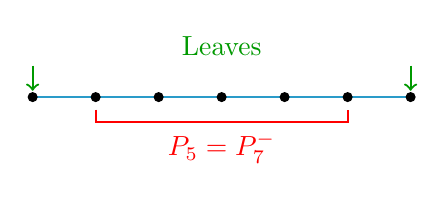
\begin{tikzpicture}[scale=0.8]
        \draw[cyan!80!black, thick] (0,0)--(6,0);
        \foreach \i in {0,...,6} \filldraw (\i,0) circle (2pt);
        
        % Bracket for T^-
        \draw[thick, red] (1,-0.2) -- (1,-0.4) -- (5,-0.4) -- (5,-0.2);
        \node[red, below] at (3,-0.4) {$P_5 = P_7^-$};
        
        % Arrows for leaves
        \draw[->, green!60!black, thick] (0, 0.5) -- (0, 0.1);
        \draw[->, green!60!black, thick] (6, 0.5) -- (6, 0.1);
        \node[green!60!black, above] at (3, 0.5) {Leaves};
    \end{tikzpicture}
    \end{center}

    \item[2)] If $T=K_{1,n}$ the complete bipartite graph, then $T^-=K_1=E_1$ consists of one vertex only:
    \begin{center}
    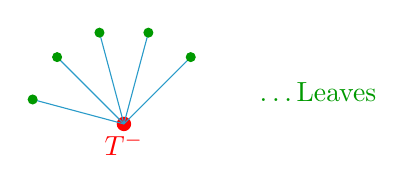
\begin{tikzpicture}[scale=0.8]
        \coordinate (c) at (0,0);
        \filldraw[red] (c) circle (3pt) node[below, red] {$T^-$};
        
        \foreach \i in {1,...,5} {
            \coordinate (l\i) at ({15+\i*30}:1.5);
            \draw[cyan!80!black] (c)--(l\i);
            \filldraw[green!60!black] (l\i) circle (2pt);
        }
        \node[green!60!black, right] at (2, 0.5) {\dots Leaves};
    \end{tikzpicture}
    \end{center}
\end{enumerate}
\end{example}

% 3.7 Lemma
\begin{lemma}
Any tree of order $n$ has exactly $n-1$ edges.
\end{lemma}

\begin{proof}
We proceed by induction on $|T|$.
If $|T|=1$, then $T=K_1$, which has zero edges and the claim holds.
Now assume we know that any tree of order $n$ has exactly $n-1$ many edges and consider $T$ of order $n+1$ arbitrary.
By Lemma 3.4, $T$ has a leaf $u$. Clearly, $T-u$ is still connected and of order $n$, whence $T-u$ has exactly $n-1$ edges.
As $u$ was a leaf in $T$, $T$ has exactly one edge more than $T-u$, whence
\[ \|T\| = n = (n+1)-1, \text{ as desired.} \qedhere \]
\end{proof}

% 3.8 Corollary
\begin{corollary}
A forest of order $n$, consisting of $k$-many connected components, has exactly $n-k$ many edges.
\end{corollary}

We will now see that given a graph $G$ is connected, Lemma 3.7 is not only a necessary, but even a sufficient condition for $G$ to be a tree.

% 3.9 Theorem
\begin{theorem}
A graph $G$ of order $n$ is a tree iff it is connected and has exactly $n-1$ many edges.
\end{theorem}

\begin{proof}
``$\Rightarrow$'' Clear by definition of a tree and Lemma 3.7.

``$\Leftarrow$'' Assume $G$ is connected of order $n$ and contains exactly $n-1$ many edges. If $G$ contains a cycle, take any edge $e_1$ within the cycle and consider $G-e_1$. Then $G-e_1$ is still connected and of order $n$. If $G-e_1$ still contains a cycle, we proceed likewise and after $k \le n-1$ many steps we obtain a graph $G-\{e_1, e_2, \dots, e_k\}$ which is of order $n$, connected and without cycles, whence it is a tree. But $G-\{e_1, \dots, e_k\}$ has $(n-1)-k < n-1$ many edges, contradicting Lemma 3.7.
\end{proof}

% 3.10 Theorem
\begin{theorem}
A graph of order $n$ is a tree iff it is acyclic and has $n-1$ many edges.
\end{theorem}

\begin{proof}
``$\Rightarrow$'' Clear.

``$\Leftarrow$'' Assume $G$ is of order $n$ with $n-1$ many edges and acyclic, i.e. $G$ is a forest. But by Corollary 3.8, if $G$ has $k$-many connected components then $\|G\| = n-k = n-1$, whence $k=1$ and $G$ is connected and hence a tree.
\end{proof}

% 3.11 Corollary (Summary)
\begin{corollary}[Summary]
Let $G$ be a graph of order $n$. Then TFAE:
\begin{enumerate}
    \item[1)] $G$ is connected and acyclic (i.e. a tree).
    \item[2)] $G$ is connected and has $n-1$ many edges.
    \item[3)] $G$ is acyclic and has $n-1$ many edges.
\end{enumerate}
\end{corollary}

% 3.12 Homework
\topic{Homework}
Every edge in a tree is a bridge.

% 3.13 Lemma
\begin{lemma}
For any two vertices $u,v \in V_T$ in a tree $T$, there is a unique $uv$-path.
\end{lemma}

\begin{proof}
As $T$ is connected, there clearly is a $uv$-path for any $u,v \in V_T$.
Now assume that $P_1 = (u=x_0, x_1, \dots, x_k=v)$ and $P_2 = (u=y_0, y_1, \dots, y_\ell=v)$ are two distinct $uv$-paths. Then $P_1 \cup P_2$ is again a tree.
Let $i$ be minimal s.t. $x_i \ne y_i$. Then $(P_1 \cup P_2) - y_i y_{i-1}$ is still connected, contradicting the fact that every edge in a tree is a bridge.
\end{proof}

% 3.14 Corollary
\begin{corollary}
Let $T$ be a tree and $v \in V_T$. Then $ecc(v)$ is the length of the longest path starting from $v$.
\end{corollary}

% 3.15 Lemma
\begin{lemma}
Let $T$ be a tree of order at least 2. Consider $u,v \in V_T$ s.t. $ecc(v) = d(u,v)$. Then $u$ is a leaf.
\end{lemma}

\begin{proof}
Let $P=(v=x_0, x_1, \dots, x_k=u)$ be the unique $vu$ path. If $u$ were not a leaf, then it had at least one neighbour $w \notin P$. But then $(v=x_0, x_1, \dots, x_k, w)$ would be a path starting in $v$ and longer than $P$, contradicting Corollary 3.14.
\end{proof}

% 3.16 Lemma
\begin{lemma}
Let $T$ be a tree of order at least 3. Then $C(T) = C(T^-)$.
\end{lemma}

\begin{proof}
\begin{enumerate}
    \item[1)] Show that $C(T) \subseteq T^-$, i.e. $C(T)$ contains no leaf.
    To this end, let $u$ be a leaf and $v$ its unique neighbour. As $|T| \ge 3$, $v$ is not a leaf itself and $d(u,w) = d(v,w) + 1$ for any $w \in V_T \setminus \{u\}$, whence $ecc(u) > ecc(v)$ and hence $u \notin C(T)$.
    
    \item[2)] Show that $ecc_{T^-}(v) = ecc_T(v) - 1$ for every non-leaf $v \in V_T$.
    To that end, consider an arbitrary non-leaf $v \in V_T$ and pick $u \in V_T$ s.t. $d(v,u) = ecc(v)$. By 3.15, $u$ is a leaf. Let $P$ be the unique $vu$-path in $T$ and note that $u$ is the only leaf on $P$. Hence only $u$ will be deleted from $P$ in $T^-$. As this holds for all paths in $T$ starting in $v$ of length $ecc(v)$, we obtain that $ecc_{T^-}(v) = ecc_T(v) - 1$, as desired.
    
    \item[3)] We conclude from 1) + 2) that for any vertex $v \in T^-$,
    $ecc_{T^-}(v) = ecc_T(v) - 1$, whence $v \in C(T)$ iff $v \in C(T^-)$ (and $rad(T^-) = rad(T)-1$).
\end{enumerate}
\end{proof}

% 3.17 Lemma
\begin{lemma}
Let $T$ be a tree. Then $C(T)$ is either $K_1$ or $K_2$.
\end{lemma}

\begin{proof}
We do induction on $|T|$. If $|T|=1$, then $T=K_1$ is its own center and we are done. Similarly for $|T|=2$, where $T=K_2$.
Now assume that the claim holds for all trees of order $n \ge 3$ and consider a tree $T$ with $|T|=n+1$ arbitrary.
By 3.16, we know that $C(T) = C(T^-)$. By 3.4 we know that $T$ contains at least two leaves, whence $|T^-| \le |T|-2 < n$. Hence, by I.H., $C(T) = C(T^-)$ is either $K_2$ or $K_1$ as desired.
\end{proof}

% 3.18 Lemma
\begin{lemma}
Let $T$ be a tree of order $n$ and $G$ an arbitrary graph s.t. $\delta(G) \ge n-1$. Then $G$ contains $T$ as a subgraph.
\end{lemma}

\begin{proof}
We use induction on $|T|$.
If $|T|=1$, then $T=K_1$ is a subgraph of any graph $G$.
Now assume we proved the claim for all trees of order at most $n$. Consider $T$ with $|T|=n+1$ and $G$ with $\delta(G) \ge n$ arbitrary.
Let $u$ be a leaf of $T$ and denote by $T' := T-u$. Then $|T'|=n$, whence $T'$ can be seen as a subgraph of $G$. Let $v$ be the unique neighbour of $u$ in $T$. Then $\deg_G(v) \ge \delta(G) \ge n$, but as $|T'|=n$ and $v$ cannot be its own neighbour, there exist some $u' \in G$ adjacent to $v$ and not contained in $T'$. Hence, the subgraph $(V_{T'} \cup \{u'\}, E_{T'} \cup \{vu'\})$ is the desired subgraph of $G$ isomorphic to $T$.
\end{proof}

\par\vspace{0.5cm}\noindent
\needspace{3\baselineskip}
{\large \underline{\textbf{Summary}}}
\par\vspace{0.2cm}
\begin{enumerate}
    \item[1)] A tree of order $n$ contains exactly $n-1$ edges.
    \item[2)] Any tree of order at least two contains at least two leaves.
    \item[3)] A graph of order $n$ is a tree iff it is connected of size $n-1$.
    \item[4)] A graph of order $n$ is a tree iff it is acyclic and of size $n-1$.
    \item[5)] A graph is a tree iff for any vertices $u,v$ there is a unique $uv$-path.
    \item[6)] The centre of any tree is either $K_1$ or $K_2$.
    \item[7)] Any graph $G$ contains any tree of order at most $\delta(G)+1$ as a subgraph.
\end{enumerate}

\section{Spanning Trees}

% 3.19 Definition
\begin{definition}
Let $G$ be any graph. We call a subgraph $T \subseteq G$ a \textbf{\color{red}spanning tree} for $G$ if it is a tree and contains all vertices of $G$.
\end{definition}

% 3.20 Remark
\begin{remark}
From the previous chapter it is clear that a spanning tree of a graph $G$ of order $n$ has $n$ many vertices and $n-1$ many edges.
\end{remark}

% 3.21 Examples
\begin{example}
Consider the following graphs and spanning trees.
\begin{enumerate}
    \item[1)] $G = C_6$, a possible spanning tree:
    \begin{center}
    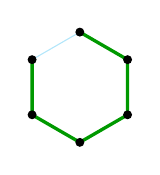
\begin{tikzpicture}[scale=0.7, baseline=(current bounding box.center)]
        % Hexagon
        \foreach \i in {1,...,6} \coordinate (v\i) at (90+60-60*\i : 1);
        
        % Base graph (faint)
        \draw[cyan!30, thin] (v1)--(v2)--(v3)--(v4)--(v5)--(v6)--(v1);
        
        % Spanning Tree (Green Path) - Missing v6-v1 edge
        \draw[green!60!black, very thick] (v1)--(v2)--(v3)--(v4)--(v5)--(v6);
        
        \foreach \i in {1,...,6} \filldraw (v\i) circle (2pt);
    \end{tikzpicture}
    \hspace{0.5cm} $\longrightarrow$ \hspace{0.5cm}
    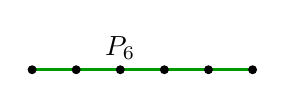
\begin{tikzpicture}[scale=0.7, baseline=(current bounding box.center)]
        % Linear Path P6
        \foreach \i in {1,...,6} \coordinate (u\i) at (\i*0.8, 0);
        \draw[green!60!black, very thick] (u1)--(u2)--(u3)--(u4)--(u5)--(u6);
        \foreach \i in {1,...,6} \filldraw (u\i) circle (2pt);
        \node[above, black] at (u3) {$P_6$};
    \end{tikzpicture}
    \end{center}

    \item[2)] $G = K_5$, possible spanning trees:
    \begin{center}
    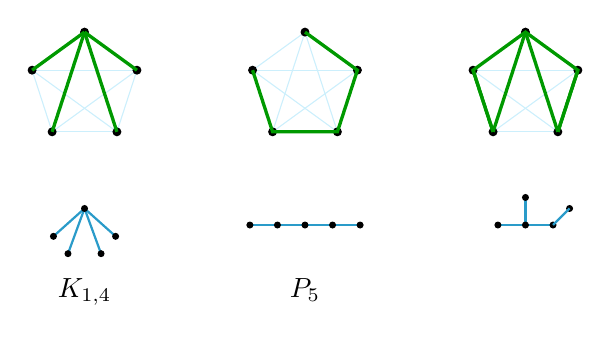
\begin{tikzpicture}[scale=0.7]
        % Define coordinates for pentagons
        \def\pentagon{
            \foreach \i in {1,...,5} \coordinate (v\i) at (90+72-72*\i : 1);
            % Faint complete graph background
            \foreach \i in {1,...,5} \foreach \j in {\i,...,5} 
                \draw[cyan!20, thin] (v\i) -- (v\j);
            \foreach \i in {1,...,5} \filldraw (v\i) circle (2pt);
        }

        % --- Column 1: Star K1,4 ---
        \begin{scope}[xshift=0cm]
            \pentagon
            % Green Edges (Star at top v1)
            \draw[green!60!black, very thick] (v1)--(v2);
            \draw[green!60!black, very thick] (v1)--(v3);
            \draw[green!60!black, very thick] (v1)--(v4);
            \draw[green!60!black, very thick] (v1)--(v5);
            
            % Abstract drawing below
            \begin{scope}[yshift=-2.5cm]
                \coordinate (c) at (0,0.3);
                \foreach \a in {200, 240, 300, 340} 
                    \draw[cyan!80!black, thick] (c) -- (\a:0.6);
                \foreach \a in {200, 240, 300, 340} 
                    \filldraw (\a:0.6) circle (1.5pt);
                \filldraw (c) circle (1.5pt);
                \node[below] at (0,-0.8) {$K_{1,4}$};
            \end{scope}
        \end{scope}

        % --- Column 2: Path P5 ---
        \begin{scope}[xshift=4cm]
            \pentagon
            % Green Edges (Path around perimeter)
            \draw[green!60!black, very thick] (v1)--(v2)--(v3)--(v4)--(v5);
            
            % Abstract drawing below
            \begin{scope}[yshift=-2.5cm]
                \draw[cyan!80!black, thick] (-1,0) -- (1,0);
                \foreach \x in {-1, -0.5, 0, 0.5, 1} \filldraw (\x,0) circle (1.5pt);
                \node[below] at (0,-0.8) {$P_5$};
            \end{scope}
        \end{scope}

        % --- Column 3: Branched Tree (Y-shape) ---
        \begin{scope}[xshift=8cm]
            \pentagon
            % Green Edges (Branched)
            % v1 connected to v2, v5. v2 connected to v3. v5 connected to v4.
            % Path v3-v2-v1-v5-v4
            \draw[green!60!black, very thick] (v3)--(v2)--(v1)--(v5)--(v4);
            % Wait, let's look at the notes "branch" drawing again.
            % It looks like Top connected to BotLeft and BotRight.
            % BotLeft connected to Left. BotRight connected to Right.
            % Let's draw that structure on the pentagon.
            \draw[green!60!black, very thick] (v2)--(v3); % Left to BotLeft
            \draw[green!60!black, very thick] (v3)--(v1); % BotLeft to Top
            \draw[green!60!black, very thick] (v1)--(v4); % Top to BotRight
            \draw[green!60!black, very thick] (v4)--(v5); % BotRight to Right
            
            % Abstract drawing below (T-shape/Y-shape)
            \begin{scope}[yshift=-2.5cm]
                \draw[cyan!80!black, thick] (0,0) -- (0,0.5); % Stem
                \draw[cyan!80!black, thick] (-0.5,0) -- (0.5,0); % Bar
                \filldraw (0,0) circle (1.5pt); \filldraw (0,0.5) circle (1.5pt);
                \filldraw (-0.5,0) circle (1.5pt); \filldraw (0.5,0) circle (1.5pt);
                \filldraw (0.8,0.3) circle (1.5pt); \draw[cyan!80!black, thick] (0.5,0) -- (0.8,0.3); % Extra branch
            \end{scope}
        \end{scope}
    \end{tikzpicture}
    \end{center}
\end{enumerate}
\end{example}

% 3.22 Lemma
\begin{lemma}
Every connected graph contains at least one spanning tree.
\end{lemma}

\begin{proof}
Assume $G$ is connected and let $T$ be a subgraph of $G$ of maximal order s.t. $T$ is a tree. We need to show that $V_T = V_G$.
Otherwise, as $G$ is connected, there is some vertex $u \in V_G \setminus V_T$ which is adjacent to some vertex $v \in V_T$. Now, consider the new subgraph $\hat{T} = (V_T \cup \{u\}, E_T \cup \{uv\})$. As $\deg_{\hat{T}}(u)=1$, $u$ is not contained in any cycles in $\hat{T}$, whence $\hat{T}$ is still a tree. As this contradicts maximality of $|T|$, we conclude that $T$ must contain all vertices of $G$, whence it is a spanning tree for $G$.
\end{proof}

% 3.24 Definition

\begin{definition}
A function $w: E_G \to \mathbb{R}$ is called a \textbf{\color{red}weight function} on $G$.
A graph $G$ together with a weight function (i.e. the triple $(V_G, E_G, w)$) is called a \textbf{\color{red}weighted graph}.
\end{definition}

% 3.25 Example - Visualisation
\begin{example}[Visualisation]
    

We visualise the weighting of a graph by denoting the weight $w(e)$ on top of the edge $e$, e.g.

\begin{center}
\begin{tikzpicture}[
    % Define specific styles to match the drawing
    city/.style={
        ellipse,
        draw=black,
        thick,
        text=blue!90!black, % Blue text
        font=\sffamily\large,
        inner sep=3pt,
        align=center
    },
    route/.style={
        draw=cyan,
        thick
    },
    label_dist/.style={
        fill=white,    % White background covers the line behind the text
        text=black,
        font=\sffamily,
        sloped,        % Rotates the text to follow the line
        inner sep=2pt
    }
]

    % --- Coordinates / Nodes ---
    % Central Hub
    \node[city] (cairo) at (0,0) {Cairo};
    
    % North / West
    \node[city] (alex) at (-2, 3.5) {Alex};
    \node[city] (fayoum) at (-3.5, -1.5) {Fayoum};
    
    % East / Sinai
    \node[city] (rassudr) at (3.5, 2.0) {RasSudr};
    \node[city] (dahab) at (7.5, 2.0) {Dahab};
    
    % South
    \node[city] (luxor) at (1.5, -3.0) {Luxor};
    \node[city] (aswan) at (6.0, -3.5) {Aswan};

    % --- Edges and Distance Labels ---
    
    % Alex Connections
    \draw[route] (alex) -- (cairo) node[label_dist, midway, above] {181};
    \draw[route] (alex) -- (rassudr) node[label_dist, midway, above] {336};
    
    % Cairo Connections
    \draw[route] (cairo) -- (fayoum) node[label_dist, midway, above] {93};
    \draw[route] (cairo) -- (rassudr) node[label_dist, midway, above] {160};
    \draw[route] (cairo) -- (dahab) node[label_dist, pos=0.65, above] {361};
    \draw[route] (cairo) -- (luxor) node[label_dist, midway, below] {502};
    \draw[route] (cairo) -- (aswan) node[label_dist, pos=0.6, above] {682};
    
    % Other Connections
    \draw[route] (rassudr) -- (dahab) node[label_dist, midway, above] {200};
    \draw[route] (luxor) -- (aswan) node[label_dist, midway, above] {180};

\end{tikzpicture}
\end{center}
Here the weight function of an edge $e=uv$ is given by the (birds eye) distance between $u$ and $v$.
\end{example}

% 3.26 Example
\begin{example}
Consider the following weighted graph.
\begin{center}
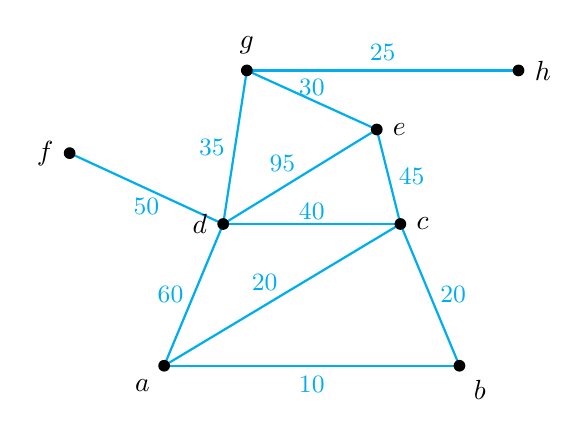
\begin{tikzpicture}[
    scale=1.5,
    node_style/.style={circle, fill=black, inner sep=1.5pt},
    edge_style/.style={cyan, thick},
    weight_style/.style={cyan, font=\small}
]
    % Coordinates
    \coordinate (a) at (0,0);
    \coordinate (b) at (2.5,0);
    \coordinate (c) at (2,1.2);
    \coordinate (d) at (0.5,1.2);
    \coordinate (e) at (1.8,2);
    \coordinate (g) at (0.7,2.5);
    \coordinate (f) at (-0.8,1.8);
    \coordinate (h) at (3.0,2.5);

    % Edges with weights
    \draw[edge_style] (a) -- (b) node[midway, below, weight_style] {10};
    \draw[edge_style] (a) -- (d) node[midway, left, weight_style] {60};
    \draw[edge_style] (a) -- (c) node[midway, above left=-2pt, weight_style] {20};
    \draw[edge_style] (b) -- (c) node[midway, right, weight_style] {20};
    \draw[edge_style] (c) -- (d) node[midway, above=-2pt, weight_style] {40};
    \draw[edge_style] (c) -- (e) node[midway, right, weight_style] {45};
    \draw[edge_style] (d) -- (e) node[midway, above left=-2pt, weight_style] {95};
    \draw[edge_style] (d) -- (g) node[midway, left, weight_style] {35};
    \draw[edge_style] (d) -- (f) node[midway, below, weight_style] {50};
    \draw[edge_style] (g) -- (e) node[midway, above=-2pt, weight_style] {30};
    \draw[edge_style] (g) -- (h) node[midway, above, weight_style] {25};

    % Nodes and Labels
    \node[node_style, label=below left:$a$] at (a) {};
    \node[node_style, label=below right:$b$] at (b) {};
    \node[node_style, label=right:$c$] at (c) {};
    \node[node_style, label=left:$d$] at (d) {};
    \node[node_style, label=right:$e$] at (e) {};
    \node[node_style, label=above:$g$] at (g) {};
    \node[node_style, label=left:$f$] at (f) {};
    \node[node_style, label=right:$h$] at (h) {};
\end{tikzpicture}
\end{center}

We can find several spanning trees. Let's name some and compute their weight.

\vspace{0.5cm}

\begin{minipage}[t]{0.45\textwidth}
    \begin{center}
    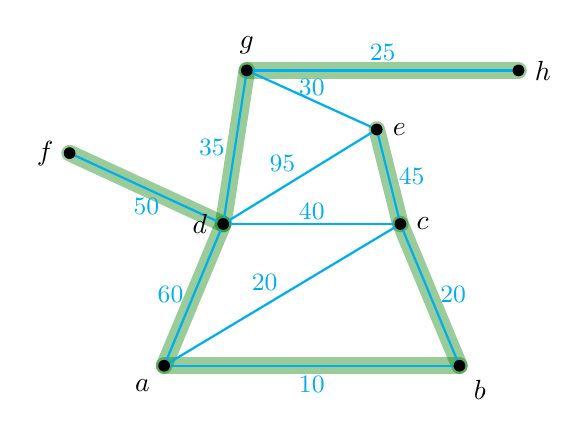
\begin{tikzpicture}[
        scale=1.5,
        node_style/.style={circle, fill=black, inner sep=1.5pt},
        edge_style/.style={cyan, thick},
        weight_style/.style={cyan, font=\small},
        highlight/.style={draw=green!50!black, opacity=0.4, line width=6pt, line cap=round}
    ]
        % Coordinates
        \coordinate (a) at (0,0);
        \coordinate (b) at (2.5,0);
        \coordinate (c) at (2,1.2);
        \coordinate (d) at (0.5,1.2);
        \coordinate (e) at (1.8,2);
        \coordinate (g) at (0.7,2.5);
        \coordinate (f) at (-0.8,1.8);
        \coordinate (h) at (3.0,2.5);

        % Green Highlights (Spanning Tree)
        % Edges: f-d, d-a, a-b, a-c, c-e, d-g, g-h
        \draw[highlight] (f) -- (d);
        \draw[highlight] (d) -- (a);
        \draw[highlight] (a) -- (b);
        \draw[highlight] (b) -- (c);
        \draw[highlight] (c) -- (e);
        \draw[highlight] (d) -- (g);
        \draw[highlight] (g) -- (h);

        % Standard Edges
        \draw[edge_style] (a) -- (b) node[midway, below, weight_style] {10};
        \draw[edge_style] (a) -- (d) node[midway, left, weight_style] {60};
        \draw[edge_style] (a) -- (c) node[midway, above left=-2pt, weight_style] {20};
        \draw[edge_style] (b) -- (c) node[midway, right, weight_style] {20};
        \draw[edge_style] (c) -- (d) node[midway, above=-2pt, weight_style] {40};
        \draw[edge_style] (c) -- (e) node[midway, right, weight_style] {45};
        \draw[edge_style] (d) -- (e) node[midway, above left=-2pt, weight_style] {95};
        \draw[edge_style] (d) -- (g) node[midway, left, weight_style] {35};
        \draw[edge_style] (d) -- (f) node[midway, below, weight_style] {50};
        \draw[edge_style] (g) -- (e) node[midway, above=-2pt, weight_style] {30};
        \draw[edge_style] (g) -- (h) node[midway, above, weight_style] {25};

        % Nodes
        \node[node_style, label=below left:$a$] at (a) {};
        \node[node_style, label=below right:$b$] at (b) {};
        \node[node_style, label=right:$c$] at (c) {};
        \node[node_style, label=left:$d$] at (d) {};
        \node[node_style, label=right:$e$] at (e) {};
        \node[node_style, label=above:$g$] at (g) {};
        \node[node_style, label=left:$f$] at (f) {};
        \node[node_style, label=right:$h$] at (h) {};
    \end{tikzpicture}
    \end{center}
    \textbf{Total weight:} \\
    $45+20+10+60+50+35+25$ \\
    $= 245$
\end{minipage}
\hfill
\begin{minipage}[t]{0.45\textwidth}
    \begin{center}
    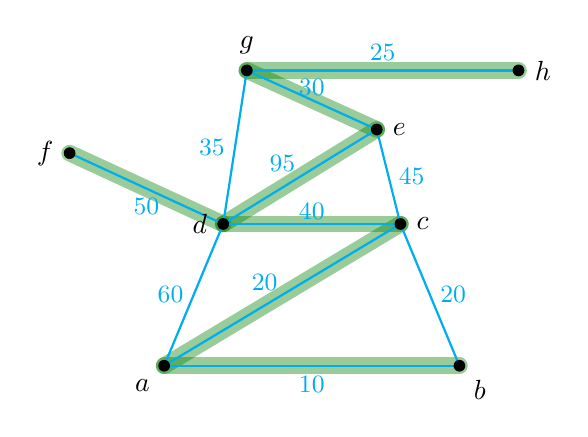
\begin{tikzpicture}[
        scale=1.5,
        node_style/.style={circle, fill=black, inner sep=1.5pt},
        edge_style/.style={cyan, thick},
        weight_style/.style={cyan, font=\small},
        highlight/.style={draw=green!50!black, opacity=0.4, line width=6pt, line cap=round}
    ]
        % Coordinates
        \coordinate (a) at (0,0);
        \coordinate (b) at (2.5,0);
        \coordinate (c) at (2,1.2);
        \coordinate (d) at (0.5,1.2);
        \coordinate (e) at (1.8,2);
        \coordinate (g) at (0.7,2.5);
        \coordinate (f) at (-0.8,1.8);
        \coordinate (h) at (3.0,2.5);

        % Green Highlights (Spanning Tree)
        % Edges: f-d, d-e, e-g, g-h, d-c, c-b, b-a
        \draw[highlight] (f) -- (d);
        \draw[highlight] (d) -- (e);
        \draw[highlight] (e) -- (g);
        \draw[highlight] (g) -- (h);
        \draw[highlight] (d) -- (c);
        \draw[highlight] (c) -- (a);
        \draw[highlight] (b) -- (a);

        % Standard Edges
        \draw[edge_style] (a) -- (b) node[midway, below, weight_style] {10};
        \draw[edge_style] (a) -- (d) node[midway, left, weight_style] {60};
        \draw[edge_style] (a) -- (c) node[midway, above left=-2pt, weight_style] {20};
        \draw[edge_style] (b) -- (c) node[midway, right, weight_style] {20};
        \draw[edge_style] (c) -- (d) node[midway, above=-2pt, weight_style] {40};
        \draw[edge_style] (c) -- (e) node[midway, right, weight_style] {45};
        \draw[edge_style] (d) -- (e) node[midway, above left=-2pt, weight_style] {95};
        \draw[edge_style] (d) -- (g) node[midway, left, weight_style] {35};
        \draw[edge_style] (d) -- (f) node[midway, below, weight_style] {50};
        \draw[edge_style] (g) -- (e) node[midway, above=-2pt, weight_style] {30};
        \draw[edge_style] (g) -- (h) node[midway, above, weight_style] {25};

        % Nodes
        \node[node_style, label=below left:$a$] at (a) {};
        \node[node_style, label=below right:$b$] at (b) {};
        \node[node_style, label=right:$c$] at (c) {};
        \node[node_style, label=left:$d$] at (d) {};
        \node[node_style, label=right:$e$] at (e) {};
        \node[node_style, label=above:$g$] at (g) {};
        \node[node_style, label=left:$f$] at (f) {};
        \node[node_style, label=right:$h$] at (h) {};
    \end{tikzpicture}
    \end{center}
    \textbf{Total weight:} \\
    $10+20+40+50+95+30+25$ \\
    $= 270$
\end{minipage}
\end{example}

% 3.27 Definition
\begin{definition}
Let $(G,w)$ be a connected weighted tree. A \textbf{\color{red}minimum-weight spanning tree} $T$ is a spanning tree of $G$ s.t. the sum of the weights of its edges is minimal among all possible spanning trees of $G$, i.e. if $\tilde{T}$ is another spanning tree, then $\sum_{e \in E_T} w(e) \le \sum_{e \in E_{\tilde{T}}} w(e)$.
\end{definition}

Now how can we find a minimal spanning tree effectively?
Consider the following algorithm:

% 3.28 Kruskal's Algorithm
\topic{Kruskal's Algorithm (1956)}
Consider the set of vertices as a forest $F=(V_G, \emptyset)$ where each vertex is a maximal subtree of $F$. Let $E := E_G$.

\textbf{While} ($F$ is not a tree $\land \ E \ne \emptyset$)
\begin{itemize}
    \item Pick $e \in E$ of minimal weight. Let $E := E \setminus \{e\}$.
    \item If $e$ connects two trees in $F$, let $E_F = E_F \cup \{e\}$.
    \item (i.e. $F+e$ is still acyclic)
\end{itemize}
This algorithm stops after at most $|E_G|$ many repetitions.

% 3.29 Example
\begin{example}
We apply the algorithm on the following weighted graph:

\begin{center}
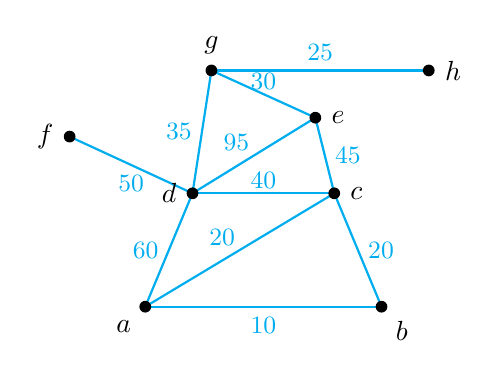
\begin{tikzpicture}[
    scale=1.2,
    node_style/.style={circle, fill=black, inner sep=1.5pt},
    edge_style/.style={cyan, thick},
    weight_style/.style={cyan, font=\small}
]
    % Coordinates
    \coordinate (a) at (0,0);
    \coordinate (b) at (2.5,0);
    \coordinate (c) at (2,1.2);
    \coordinate (d) at (0.5,1.2);
    \coordinate (e) at (1.8,2);
    \coordinate (g) at (0.7,2.5);
    \coordinate (f) at (-0.8,1.8);
    \coordinate (h) at (3.0,2.5);

    % Edges with weights
    \draw[edge_style] (a) -- (b) node[midway, below, weight_style] {10};
    \draw[edge_style] (a) -- (d) node[midway, left, weight_style] {60};
    \draw[edge_style] (a) -- (c) node[midway, above left=-2pt, weight_style] {20};
    \draw[edge_style] (b) -- (c) node[midway, right, weight_style] {20};
    \draw[edge_style] (c) -- (d) node[midway, above=-2pt, weight_style] {40};
    \draw[edge_style] (c) -- (e) node[midway, right, weight_style] {45};
    \draw[edge_style] (d) -- (e) node[midway, above left=-2pt, weight_style] {95};
    \draw[edge_style] (d) -- (g) node[midway, left, weight_style] {35};
    \draw[edge_style] (d) -- (f) node[midway, below, weight_style] {50};
    \draw[edge_style] (g) -- (e) node[midway, above=-2pt, weight_style] {30};
    \draw[edge_style] (g) -- (h) node[midway, above, weight_style] {25};

    % Nodes and Labels
    \node[node_style, label=below left:$a$] at (a) {};
    \node[node_style, label=below right:$b$] at (b) {};
    \node[node_style, label=right:$c$] at (c) {};
    \node[node_style, label=left:$d$] at (d) {};
    \node[node_style, label=right:$e$] at (e) {};
    \node[node_style, label=above:$g$] at (g) {};
    \node[node_style, label=left:$f$] at (f) {};
    \node[node_style, label=right:$h$] at (h) {};
\end{tikzpicture}
\end{center}

Let us mark edges we add to $F$ green and the ones we disregard, red.

\vspace{1em}

% --- The Algorithm Steps (Wrapped in a minipage to keep them together) ---
\noindent
\begin{minipage}{\textwidth}
    % Common TikZ settings for the small graphs
    \tikzset{
        tiny_graph/.style={
            scale=0.85, % INCREASED SCALE FOR 2 COLUMNS
            baseline=(current bounding box.center),
            node_style/.style={circle, fill=black, inner sep=1.5pt},
            edge_style/.style={cyan, thick},
            weight_style/.style={cyan, font=\tiny}, 
            highlight/.style={draw=green!50!black, opacity=0.4, line width=4pt, line cap=round},
            highlightred/.style={draw=red!100!black, opacity=1, line width=4pt, line cap=round}
        }
    }

    % --- ROW 1 (Steps 1 & 2) ---
    \begin{minipage}[t]{0.48\textwidth}
        \textbf{1)} $E=E_G, E_F=\emptyset$ \\
        \begin{tikzpicture}[tiny_graph]
            \coordinate (a) at (0,0); \coordinate (b) at (2.5,0); \coordinate (c) at (2,1.2);
            \coordinate (d) at (0.5,1.2); \coordinate (e) at (1.8,2); \coordinate (g) at (0.7,2.5);
            \coordinate (f) at (-0.8,1.8); \coordinate (h) at (3.0,2.5);
            \draw[edge_style] (a)--(b) (a)--(d) (a)--(c) (b)--(c) (c)--(d) (c)--(e) (d)--(e) (d)--(g) (d)--(f) (g)--(e) (g)--(h);
            \foreach \p in {a,b,c,d,e,g,f,h} \node[node_style] at (\p) {};
        \end{tikzpicture}
    \end{minipage}%
    \hfill
    \begin{minipage}[t]{0.48\textwidth}
        \textbf{2)} $E=E-\{ab\}, E_F=\{ab\}$ \\
        \begin{tikzpicture}[tiny_graph]
            \coordinate (a) at (0,0); \coordinate (b) at (2.5,0); \coordinate (c) at (2,1.2);
            \coordinate (d) at (0.5,1.2); \coordinate (e) at (1.8,2); \coordinate (g) at (0.7,2.5);
            \coordinate (f) at (-0.8,1.8); \coordinate (h) at (3.0,2.5);
            \draw[highlight] (a)--(b);
            \draw[edge_style] (a)--(b) (a)--(d) (a)--(c) (b)--(c) (c)--(d) (c)--(e) (d)--(e) (d)--(g) (d)--(f) (g)--(e) (g)--(h);
            \foreach \p in {a,b,c,d,e,g,f,h} \node[node_style] at (\p) {};
        \end{tikzpicture}
    \end{minipage}
    
    \vspace{1.5em}

    % --- ROW 2 (Steps 3 & 4) ---
    \begin{minipage}[t]{0.48\textwidth}
        \textbf{3)} $E=E-\{ac\}, E_F=E_F \cup \{ac\}$ \\
        \begin{tikzpicture}[tiny_graph]
            \coordinate (a) at (0,0); \coordinate (b) at (2.5,0); \coordinate (c) at (2,1.2);
            \coordinate (d) at (0.5,1.2); \coordinate (e) at (1.8,2); \coordinate (g) at (0.7,2.5);
            \coordinate (f) at (-0.8,1.8); \coordinate (h) at (3.0,2.5);
            \draw[highlight] (a)--(b) (a)--(c);
            \draw[edge_style] (a)--(b) (a)--(d) (a)--(c) (b)--(c) (c)--(d) (c)--(e) (d)--(e) (d)--(g) (d)--(f) (g)--(e) (g)--(h);
            \foreach \p in {a,b,c,d,e,g,f,h} \node[node_style] at (\p) {};
        \end{tikzpicture}
    \end{minipage}%
    \hfill
    \begin{minipage}[t]{0.48\textwidth}
        \textbf{4)} $E=E-\{bc\}, E_F=E_F$ \\
        \begin{tikzpicture}[tiny_graph]
            \coordinate (a) at (0,0); \coordinate (b) at (2.5,0); \coordinate (c) at (2,1.2);
            \coordinate (d) at (0.5,1.2); \coordinate (e) at (1.8,2); \coordinate (g) at (0.7,2.5);
            \coordinate (f) at (-0.8,1.8); \coordinate (h) at (3.0,2.5);
            \draw[highlight] (a)--(b) (a)--(c);
            \draw[highlightred] (b)--(c);
            \draw[edge_style] (a)--(b) (a)--(d) (a)--(c) (b)--(c) (c)--(d) (c)--(e) (d)--(e) (d)--(g) (d)--(f) (g)--(e) (g)--(h);
            \foreach \p in {a,b,c,d,e,g,f,h} \node[node_style] at (\p) {};
        \end{tikzpicture}
    \end{minipage}

    \vspace{1.5em}

    % --- ROW 3 (Steps 5 & 6) ---
    \begin{minipage}[t]{0.48\textwidth}
        \textbf{5)} $E=E-\{gh\}, E_F=E_F \cup \{gh\}$ \\
        \begin{tikzpicture}[tiny_graph]
            \coordinate (a) at (0,0); \coordinate (b) at (2.5,0); \coordinate (c) at (2,1.2);
            \coordinate (d) at (0.5,1.2); \coordinate (e) at (1.8,2); \coordinate (g) at (0.7,2.5);
            \coordinate (f) at (-0.8,1.8); \coordinate (h) at (3.0,2.5);
            \draw[highlight] (a)--(b) (a)--(c) (g)--(h);
            \draw[highlightred] (b)--(c);
            \draw[edge_style] (a)--(b) (a)--(d) (a)--(c) (b)--(c) (c)--(d) (c)--(e) (d)--(e) (d)--(g) (d)--(f) (g)--(e) (g)--(h);
            \foreach \p in {a,b,c,d,e,g,f,h} \node[node_style] at (\p) {};
        \end{tikzpicture}
    \end{minipage}%
    \hfill
    \begin{minipage}[t]{0.48\textwidth}
        \textbf{6)} $E=E-\{ge\}, E_F=E_F \cup \{ge\}$ \\
        \begin{tikzpicture}[tiny_graph]
            \coordinate (a) at (0,0); \coordinate (b) at (2.5,0); \coordinate (c) at (2,1.2);
            \coordinate (d) at (0.5,1.2); \coordinate (e) at (1.8,2); \coordinate (g) at (0.7,2.5);
            \coordinate (f) at (-0.8,1.8); \coordinate (h) at (3.0,2.5);
            \draw[highlight] (a)--(b) (a)--(c) (g)--(h) (g)--(e);
            \draw[highlightred] (b)--(c);
            \draw[edge_style] (a)--(b) (a)--(d) (a)--(c) (b)--(c) (c)--(d) (c)--(e) (d)--(e) (d)--(g) (d)--(f) (g)--(e) (g)--(h);
            \foreach \p in {a,b,c,d,e,g,f,h} \node[node_style] at (\p) {};
        \end{tikzpicture}
    \end{minipage}

    \vspace{1.5em}

    % --- ROW 4 (Steps 7 & 8) ---
    \begin{minipage}[t]{0.48\textwidth}
        \textbf{7)} $E=E-\{gd\}, E_F=E_F \cup \{gd\}$ \\
        \begin{tikzpicture}[tiny_graph]
            \coordinate (a) at (0,0); \coordinate (b) at (2.5,0); \coordinate (c) at (2,1.2);
            \coordinate (d) at (0.5,1.2); \coordinate (e) at (1.8,2); \coordinate (g) at (0.7,2.5);
            \coordinate (f) at (-0.8,1.8); \coordinate (h) at (3.0,2.5);
            \draw[highlight] (a)--(b) (a)--(c) (g)--(h) (g)--(e) (g)--(d);
            \draw[highlightred] (b)--(c);
            \draw[edge_style] (a)--(b) (a)--(d) (a)--(c) (b)--(c) (c)--(d) (c)--(e) (d)--(e) (d)--(g) (d)--(f) (g)--(e) (g)--(h);
            \foreach \p in {a,b,c,d,e,g,f,h} \node[node_style] at (\p) {};
        \end{tikzpicture}
    \end{minipage}%
    \hfill
    \begin{minipage}[t]{0.48\textwidth}
        \textbf{8)} $E=E-\{cd\}, E_F=E_F \cup \{cd\}$ \\
        \begin{tikzpicture}[tiny_graph]
            \coordinate (a) at (0,0); \coordinate (b) at (2.5,0); \coordinate (c) at (2,1.2);
            \coordinate (d) at (0.5,1.2); \coordinate (e) at (1.8,2); \coordinate (g) at (0.7,2.5);
            \coordinate (f) at (-0.8,1.8); \coordinate (h) at (3.0,2.5);
            \draw[highlight] (a)--(b) (a)--(c) (g)--(h) (g)--(e) (g)--(d) (c)--(d);
            \draw[highlightred] (b)--(c);
            \draw[edge_style] (a)--(b) (a)--(d) (a)--(c) (b)--(c) (c)--(d) (c)--(e) (d)--(e) (d)--(g) (d)--(f) (g)--(e) (g)--(h);
            \foreach \p in {a,b,c,d,e,g,f,h} \node[node_style] at (\p) {};
        \end{tikzpicture}
    \end{minipage}

    \vspace{1.5em}

    % --- ROW 5 (Steps 9 & 10) ---
    \begin{minipage}[t]{0.48\textwidth}
        \textbf{9)} $E=E-\{ce\}, E_F=E_F$ \\
        \begin{tikzpicture}[tiny_graph]
            \coordinate (a) at (0,0); \coordinate (b) at (2.5,0); \coordinate (c) at (2,1.2);
            \coordinate (d) at (0.5,1.2); \coordinate (e) at (1.8,2); \coordinate (g) at (0.7,2.5);
            \coordinate (f) at (-0.8,1.8); \coordinate (h) at (3.0,2.5);
            \draw[highlight] (a)--(b) (a)--(c) (g)--(h) (g)--(e) (g)--(d) (c)--(d);
            \draw[highlightred] (b)--(c) (e)--(c);
            \draw[edge_style] (a)--(b) (a)--(d) (a)--(c) (b)--(c) (c)--(d) (c)--(e) (d)--(e) (d)--(g) (d)--(f) (g)--(e) (g)--(h);
            \foreach \p in {a,b,c,d,e,g,f,h} \node[node_style] at (\p) {};
        \end{tikzpicture}
    \end{minipage}%
    \hfill
    \begin{minipage}[t]{0.48\textwidth}
        \textbf{10)} $E=E-\{df\}, E_F=E_F \cup \{df\}$ \\
        \begin{tikzpicture}[tiny_graph]
            \coordinate (a) at (0,0); \coordinate (b) at (2.5,0); \coordinate (c) at (2,1.2);
            \coordinate (d) at (0.5,1.2); \coordinate (e) at (1.8,2); \coordinate (g) at (0.7,2.5);
            \coordinate (f) at (-0.8,1.8); \coordinate (h) at (3.0,2.5);
            \draw[highlight] (a)--(b) (a)--(c) (g)--(h) (g)--(e) (g)--(d) (c)--(d) (f)--(d);
            \draw[highlightred] (b)--(c) (e)--(c);
            \draw[edge_style] (a)--(b) (a)--(d) (a)--(c) (b)--(c) (c)--(d) (c)--(e) (d)--(e) (d)--(g) (d)--(f) (g)--(e) (g)--(h);
            \foreach \p in {a,b,c,d,e,g,f,h} \node[node_style] at (\p) {};
        \end{tikzpicture}
    \end{minipage}
    
\end{minipage}

\vspace{1em}

Here the algorithm stops, as 
$F = (V_G, E_F)$ with $E_F = \{ab, ac, gh, eg, dg, cd, df\}$ 
is a single tree whence the conditions in 
the while loop are violated.\\
(The output is the spanning tree $F$. Note that the second condition 
in the while loop was still valid, as $E = \{ad, de\} \neq \emptyset$).
\end{example}

% 3.30 Theorem
\begin{theorem}
Kruskal's algorithm is correct, i.e. it always terminates and its output is a minimum-weight spanning tree.
\end{theorem}

\begin{proof}
\begin{enumerate}
    \item[1)] Termination: As after $|E_G|$-many steps the condition $E \ne \emptyset$ is violated, the algorithm always terminates.
    \item[2)] The output $F$ is a spanning tree:
    As $V_F=V_G$, it clearly contains all vertices of $G$.
    Further, in each step the regarded edge $e$ either connects two disconnected trees into one larger tree, or, if it would connect two vertices of the same subtree in $F$, is disregarded. Hence after each step, $F$ is still a forest, i.e. acyclic.
    It remains to show that $F$ is connected. If the algorithm stops because $F$ is a tree, then it is clearly connected. If it stops because we went through all the edges, then any edge of $G$ not contained in $F$ would connect two vertices of the same connected component. Thus $F$ has as many connected components as $G$, which is one, as $G$ is connected.
    \item[3)] $F$ is a minimum-weight spanning tree.
    Aiming for a contradiction, assume this is not the case. Let $\{e_1, \dots, e_{n-1}\}$ be all the edges in $F$, enumerated in the order they were added to $F$ by the algorithm.
    Among all possible minimum-weight spanning trees, let $T$ be one that agrees with $F$ on the largest initial segment of $(e_1, \dots, e_{n-1})$, i.e. if $k$ is the smallest index s.t. $e_{k+1} \notin T$, then there is no minimum-weight spanning tree which contains $\{e_1, \dots, e_{k+1}\}$.
    As by assumption $F$ is not minimum-weight, we have $k < n-1$.
    As $T$ is a spanning tree which does not contain $e_{k+1}$, we know that $T+e_{k+1}$ contains a cycle $C$. As $F$ did not contain cycles, there is one edge $e \in C \subseteq T$ which is not in $F$.
    Now $T+e_{k+1}-e$ is a connected graph of order $n$ and size $n-1$, whence still a spanning tree. It contains the edges $\{e_1, \dots, e_k, e_{k+1}\}$, hence it can no longer be of minimum weight. This means that $w(e_{k+1}) > w(e)$.
    But as $e \notin F$ and in particular $e \notin \{e_1, \dots, e_k\}$ this means $e$ was available at the step of the algorithm after we added $e_k$ and of less weight than $e_{k+1}$. This contradicts the assumption that the algorithm chooses the edge of minimal weight which keeps $F$ acyclic. \qedhere
\end{enumerate}
\end{proof}

% 3.31 Lemma
\begin{lemma}
If $G$ is a connected weighted graph s.t. distinct edges have distinct weights, then there is a unique minimum-weight spanning tree.
\end{lemma}

\begin{proof}
Homework.
\end{proof}